Le but de cette section est d'analsyer quels sont les besions des différents utilisateurs et de trouver quelle est la meilleure manière d'y répondre. Un autre point très important est le détails des choix technologiques. Je vais donc tous les passer en revue et les expliquer.
\section{Besoins}

Dans un premier temps, il convient d'identifier quels seront les différents types d'utilisateurs de cette plateforme de quiz. Il y a selon moi deux types bien distinct d'utilisateurs :
\begin{itemize}
    \item Les étudiants
    \item Les professeurs
\end{itemize}

Les premiers utilisent cette plateforme afin de répondre à des quizs. La forme de ces derniers peuvent varier entre un simple quiz pour valider un devoir, un drill dans le but de réviser un examen ou finalement l'examen en lui-même. Ils ont donc besoin d'une interface où ils peuvent voir et choisir un quiz parmi tous ceux dont l'accès leurs est autorisé. Il doit pouvoir répondre au quiz et dans le cadre d'un examen ou d'un devoir il doit pouvoir le rendre. Il doit également pouvoir naviguer dans le quiz.

Les professeurs quant à eux ont des besoins bien différents. Ils veulent principalement créer des quizs avec des questions de plusieurs types tels que un QCM, des textes à trous ou encore des questions de code. Ils doivent également pouvoir regrouper leurs étudiants en différentes classes et autoriser cette classe à répondre à certains quizs. Dernièrement, ils ont besoin de pouvoir corriger automatiquement certaines questions comme les QCM.

%TODO : Mettre digramme



\section{Technologies}
Dans cette sous-section, je vais détailler les différentes technologies qui seront utilisées dans ce projet.
\subsection{Technologies présentes dans l'application}
Je vais brièvement rappeler les choix technologiques qui ont déjà été pris pour ce projet :
\begin{itemize}
    \item Pour le SGBD : MySQL.
    \item Pour le backend : le framework PHP, Laravel version 8.
    \item Pour le frontend : le framework javascript, Vue.js version 2.
    \item Pour le style de l'application: Bootstrap et CSS
    \item Pour la connexion à l'application (SSO) : Shibboleth
    \item Système de gestion de version : Github
\end{itemize}

\subsection{Choix technologiques}
Je vais maintenant expliquer et détailler chaque technologie qui sera utilisée au cours de ce projet.

\subsection{MySQL}
MySQL est un système de gestion de bases de données relationnelles (SGBDR) open source et très répandu. Il est bien souvent utilisé dans le développement d'applications ou de sites webs pour stocker et récupérer efficacement des données. MySQL utilise le langage de requête SQL pour travailler avec les données. Ce langage permet des fonctionnalités telles que la création de tables, l'insertion, la suppression et la mise à jour des données. Il permet également des fonctionnalités plus avancées comme les jointures qui permettent de récupérer et combiner les données provenant de plusieurs tables différentes mais liées. Ce SGBD a été dévelopé dans le but d'avoir des performances élevées. Sa fiabilité ainsi que sa simplicité à l'utilisation en ont fait l'un des leader dans le monde des SGBD.

Comme le montre le site web de ranking de SGBD \href{https://db-engines.com/en/ranking}{DB-engines}, MySQL est le deuxième SGBD le plus populaire au monde. On voit également que sa place est plutôt fixe car le podium n'a pas bougé depuis plus d'un an.
\begin{center} %TODO : Changer la taille de cette image
    \begin{figure}[H]
        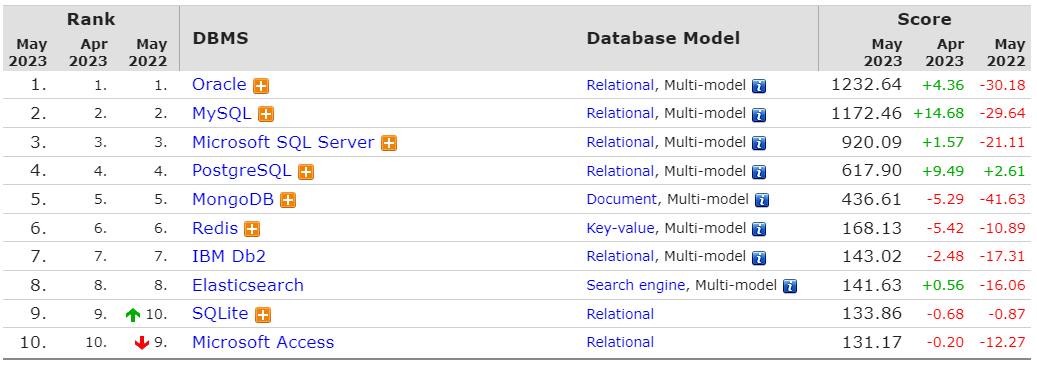
\includegraphics[width=10cm]{./assets/figures/MySQLPopularity.png}
        \caption{Popularité des différents SGBD dans le monde \label{MySQLPopularity.png}}
    \end{figure}
\end{center}
On voit également sur ce classement que les SGBD les plus populaires ont des scores assez similaire et ont tous deux de la marge sur leur concurent qui occupe la troisième place. Oracle étant un SGBDR légèrement plus populaire que MySQL, il aurait pu être intéressant de choisir ce SGBD.

\begin{center}
    \begin{figure}[H]%TODO : Changer la taille de cette image
        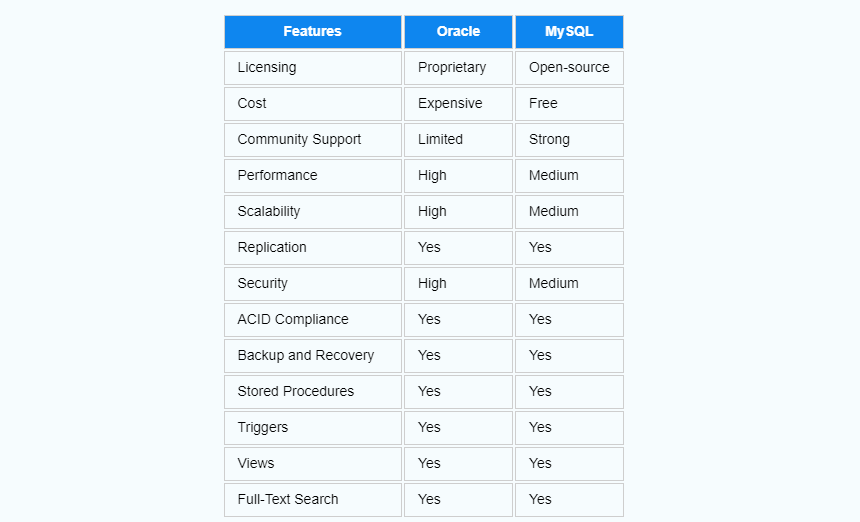
\includegraphics[width=\textwidth]{./assets/figures/OracleVsMySql.png}
        \caption{Comparaison entre Oracle et MySql \label{OracleVsMySql.png}}
    \end{figure}
\end{center}
Cependant comme montré dans l'article du site \href{https://www.integrate.io/blog/oracle-vs-mysql/#:~:text=Oracle%20supports%20distributed%20databases%20while,Oracle%20requires%20a%20licensing%20fee.}{Integrate.io} les avantages sont minimes (des performances un peu meilleures et un sécuritée accrue). La license Oracle étant cependant très onéreuse, Oracle ne fait pas un bon candidat dans le cadre de ce travail de Bachelor.

C'est pourquoi j'ai décidé de rester sur la version 8.0 de MySQL. De plus, grace au framework Laravel il est extrêment simple de changer de SGBD. Il suffit de modifier le fichier de configuration.

\subsection{Laravel}
Laravel est un framework web open-source, écrit en PHP, offrant une structure solide et élégante pour la création d'application et de site web. Le but principal de ce framework est de simplifier la création et le développement d'application grâce à des fonctionnalités intégrées au framework. On y retrouve la gestion de routes, les sessions, l'authentification des utilisateurs ainsi que la gest de la base de données.
Laravel fourni un ORM (Object Relational Mapping), appelé Eloquent permettant de gérer toutes les intercations avec la base de données. Il permet également de choisir avec quel type de SGBD nous souhaitons travailler et de changer ce dernier très rapidement grâce à des fichiers de configuration.
Il propose un pattern architechturale très utilisé, le Modèle-Vue-Controller.
\begin{center}
    \begin{figure}[H]%TODO : Changer la taille de cette image
        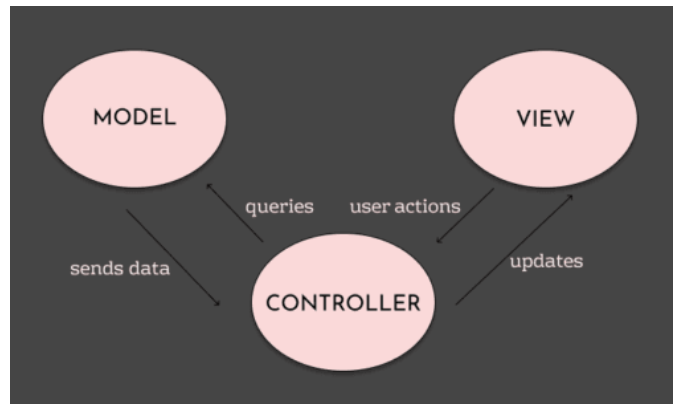
\includegraphics[width=\textwidth]{./assets/figures/MVCExplanation.png}
        \caption{Représentation du MVC \label{MVCExplanation.png}}
    \end{figure}
\end{center}

Sur cette capture, tirée du site \href{https://pusher.com/blog/laravel-mvc-use/#what-is-mvc}{Pusher}, on peut voir les trois parties de ce système et comment elles interagissent.
\begin{itemize}
    \item Le Modèle est la partie responsable de la gestion des données ainsi que de la logique métier. C'est la seule partie du pattern qui interagit avec la base de données. Il représente les structures de données, et fourni au Controller des méthodes pour manipuler les données.
    \item La vue est la partie qui gère de l'interface utilisateur. Elle affiche les données et permet également de récupérer les informations saisies par l'utilisateur notamment au travers de formulaires.
    \item Le Controller est la partie qui lie le Modèle et la Vue. Il réagit aux inputs de l'utilisateur qui sont transmis par la Vue et va interroger, si nécessaire, le Modèle afin d'y metter à jours ou récupérer des données. C'est également lui qui détermine quelle est la Vue à afficher à l'utilisateur. C'est le responsable de la logique de l'application.
\end{itemize}
Le MVC permet donc d'avoir une séparation distincte entre les différentes parties de notre application.

Un autre point fort de Laravel est sa gestion des middleware. Un Middleware est une sorte de filtre qui intervient lorsque les requêtes HTTP arrivent dans notre application. Cela permet notamment d'imposer qu'un utilisateur soit authentifié avant d'accéder à certaines routes ou URL. Ils offre donc un contrôle accru et centralisent la logique de certaines fonctionnalités.

Laravel est donc l'un des framework les plus populaires, simple à prendre en main avec une documentation complète et mise à jour. Il est donc le candidat idéal pour ce projet. De plus, un changement de framework imposerait une charge de travail supplémentaire bien trop conséquente.
Je vais donc utiliser la version 10 de Laravel.

\subsection{Vue.js}
Vue.js est un framework JavaScript open-source, populaire et polyvalent permettant de créer des interfaces utilisateurs. Il est principalement utilisé enpour le frontend d'applications et peut facilement être ajouté à de gros projets. Il propose une approche basé sur les composants qui permettent de créer des portions de codes réutilisable. Grâce à une liaison bidirectionnelle entre les données et l'interface, Vue.js permet de synchroniser, en temps réel, les données entrées par l'utilisateur et leur affichage.

Ce qui permet à Vue.js d'être aussi performant est l'utilisation d'un \emph{DOM} virtuel. Le \emph{DOM (Document Object Model)} est une représentation hierarchique d'un document HTML sous la forme d'un arbre. Il permet donc à des langages de programmation de modifier le style ou la forme de ce document. Cependant à chaque changement, le navigateur va mettre à jour l'interface. Cela peut grandement impacter les performances si les modifications sont très fréquentes. C'est pourquoi Vue.js utilise un \emph{DOM} virtuel ou \emph{Virtual DOM}. Il s'agit d'une copie virtuelle stockée en mémoire du \emph{DOM} réel. Lors d'une mise à jour, les changements sont stocké dans le \emph{Virtual DOM}. Vue.js va ensuite comparer le \emph{Virtual DOM} avec le \emph{DOM} réel et n'appliquer que les changements nécessaires. Cela explique pourquoi ce framework a des performances relativement élevées.

Avec Vue.js, on trouve Pinia qui est le gestionnaire d'état conseillé pour la version 3 de Vue.js. Il permet de gérer l'état de l'application et de le partager entre les différents composants. Cet outil va nous être très utile au cours de ce projet.

Une autre fonctionnalité très importante de ce framework est la capacité de créer des \emph{Singe Page Application} ou une application à page unique. Le concept dernière les SPA est que toute l'application est rendue sur une seule page. La SPA va initialement charger une page puis va dynamiquement changer son contenu en fonction des besoins et volontés de l'utilisateur. Cela permet une expérience utilisateur plus rapide et fluide qu'avec une application classique.

Les principaux concurrent du framework Vue.js sont React et Angular. Selon un sondage réalisé par \href{https://survey.stackoverflow.co/2022/#most-popular-technologies-webframe}{StackOverflow} en 2022, React est plus populaire que Vue.js et Angular.
\begin{center}
    \begin{figure}[H]%TODO : Changer la taille de cette image
        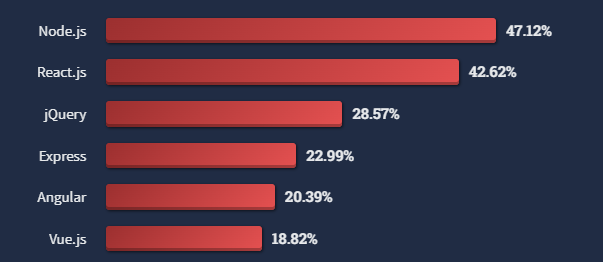
\includegraphics[width=\textwidth]{./assets/figures/VueVSReactVSAngular.png}
        \caption{Popularité des framework web \label{VueVSReactVSAngular.png}}
    \end{figure}
\end{center}

Comme Vue.js, React est un framework javascript performant et dipose d'une communauté active. Il aurait été un bon choix de technologie pour ce projet car plus utilisé dans l'industrie et disposant d'une plus grande communauté.

Cependant, comme pour Laravel, un changement de framework aurait imposé une charge de travail supplémentaire trop importante. De plus, Vue.js est plus simple à prendre en main et à utiliser que React. Il est donc plus adapté à un projet de cette envergure. Je vais donc utiliser la version 3.0 de Vue.js.

\subsection{Tailwind CSS}
Tailwind CSS est un framework CSS open-source très simple à installer et utiliser. Il favorise la création rapide d'interfaces utilisateur personnalisées. Contrairement à son principal concurrent Bootstrap, Tailwind CSS ne propose pas de composants prédéfinis. On y retrouve plutôt des classes utilitaires qui permettent de modifier rapidement le style d'un élément. Chaque classe est indépendante et ne représente qu'une fonctionnalité. Par exemple la classe "mb-4" permet d'ajouter une marge sur le bas d'un élément. Cela rend la personnalisation de l'interface utilisateur plus simple et plus rapide. On peut également créer ses propres classes utilitaires.

Un détail important de ce framework est qu'il enlève tous les styles de base des navigateurs. Cela permet d'avoir une interface utilisateur cohérente sur tous les navigateurs.

Un autre point fort de ce framework est sa communauté active. En effet, Tailwind CSS dispose d'une documentation complète et de nombreux exemples.

Les raisons qui ont fait que j'ai choisi Tailwind CSS sont sa simplicité d'utilisation, sa capacité de personnalisation. Bootstrap aurait été également un choix tout à fait valable. Cependant, pour avoir déjà travailler avec ces deux framework, j'ai une légère préférence pour Tailwind CSS.

\subsection{Keycloak}
Keycloak est une solution open-source de gestion d'identité et d'accès. Cela évite à notre application d'avoir à gérer les différents formulaires d'authentification, d'inscriptions ou de changement de mot de passes. Keycloak propose également une gestion des rôles et des permissions. Cela permet de définir des rôles pour les utilisateurs.

Dans le cadre de ce projet, tous les utilisateurs sont des membres de la HEIG-VD. Les deux choix que nous avions étaient d'utiliser Keycloak (le système de l'école) ou SWITCH edu-ID basé sur Shibboleth (actuellement utilisé dans le projet).

Le grand avantage de Keycloak est la maitrise complète de l'outil par le service informatique de l'école. Cela permet une meilleur communication et entre aide. De plus, Keycloak a déjà été utilisé sur plusieurs projets de l'école, donc sa mise en place sera simplifiée.
C'est pour ces raisons là que j'ai décidé d'utiliser Keycloak.

\subsection{Github}
Github est une plateforme web de développement collaboratif basée sur Git. Elle facilite énormément la gestion de version de notre code source. De plus, elle favorise grandement la collaboration entre les différents développeurs. Github propose notamment des fonctionnalités de gestion de projet, permettant notamment des créer des tâches et de les assigner à des personnes. Ce qui aide à avoir une meilleure vue d'ensemble du projet.

Github permet également grâce à ses \emph{Github Actions} de créer des \emph{workflows CI/CD} qui permettent d'automatiser certaines tâches. Par exemple, on peut créer un \emph{workflow} qui va automatiquement lancer les tests unitaires à chaque modification du code qui sera poussé sur la plateforme. On peut également créer des \emph{Github Actions} qui vont déployer automatiquement notre application sur un serveur.

Github est la plateforme de gestion de version la plus populaire et la plus utilisée dans le monde. Selon les statistiques de l'article de \href{https://radixweb.com/blog/github-vs-gitlab}{Radix}, Github aurait environ 56 millions d'utilisateurs contre 31 millions pour Gitlab. Avec son système de \emph{stars} et son côté social, Github est la plateforme idéale pour un projet open-source.

Toutes ces raisons font que Github est la plateforme de gestion de version que j'ai choisi pour ce projet.

\subsection{Récapitulatif des technologies}
Dans la tableau ci-dessous, vous pouvez trouver la liste de toutes les technologies qui sont utilisée dans le cadre de ce projet ainsi que leur version.
% Fais un tableau avec toutes les technologies utilisées dans le projet
\begin{center}
    \begin{tabular}{|l|l|}
        \hline
        \textbf{Technologie} & \textbf{Version} \\
        \hline
        MySQL                & 8.0              \\
        \hline
        PHP                  & 8.2.6            \\
        \hline
        Composer             & 2.5.5            \\
        \hline
        Laravel              & 10               \\
        \hline
        Node                 & 18.15.0          \\
        \hline
        NPM                  & 9.5.0            \\
        \hline
        Vue.js               & 3                \\
        \hline
        Tailwind CSS         & 3.3.1            \\
        \hline
        WSl                  & 2                \\
        \hline
        Docker               & 20.10.22         \\
        \hline
        Ubuntu               & 22.04.2 LTS      \\
        \hline
        Keycloak local       & 21.1             \\
        \hline
        Github               & -                \\
        \hline
    \end{tabular}
\end{center}
